\section{Gains et confort thermique}

La connaissance de la présence des occupants dans les différentes zones des bâtiments est comme nous l'avons déjà évoqué un pré-requis aux modèles adaptatifs (actions sur les fenêtres, les occultations et l'éclairage) et aux modèles d'usage d'électricité spécifique et de consommations d'ECS. Cette section présence comment cette présence est de surcroit exploitable pour associer des gains métaboliques à chaque zone et attribuer à chaque occupant un niveau de confort thermique évalué par les indices PMV (\textit{Predicted Mean Vote}) et PPD (\textit{Predicted Percentage Dissatisfied}). La norme ISO 7730 \cite{ISO7730} issu du travail initial de Fanger \cite{Fanger-70} est utilisé pour définir les gains métaboliques et les indicateurs de confort thermique. Nous proposons ainsi une présentation de l'algorithme implémenté dans la plateforme MASS.

Nous pouvons d'ores et déjà indiqué que comme EnergyPlus ne prend qu'un unique taux métabolique par zone, le FMU ne renverra pas des gains pour chaque occupant mais une somme pour l'ensemble des occupants présents par zone.

Les modèles d'activités (Section \ref{ActivitésLogements}) et de présence (Section \ref{PresenceBureau}) ont permit d'attribuer des scénarios stochastiques de présence dans les bâtiments pour l'ensemble des occupants. Le Tableau \ref{tab:Activités} (Page \pageref{tab:Activités}) présentait les associations entre activités et pièces ainsi que le niveau d'isolation vestimentaire $Clo$ et le taux métabolique $Met$.

Comme nous l'avions présenté lors de la présentation de la plateforme du comportement des occupants; MASS (Chapitre \ref{MASS}), l'intérêt de la co-simulation est de pouvoir faire échanger des variables entre EnergyPlus et la plateforme de modélisation des comportements des occupants. D'après la norme ISO-7730 \cite{ISO7730} nous avons besoin de variables environnementales pour le calcul des gains internes. Ces gains internes pour l'environnement sont égaux à la somme (Eq. \ref{GM}) de la perte d'énergie latente (par diffusion au travers de la peau (Eq. \ref{GM1}), par sudation (Eq. \ref{GM2}) et par respiration (Eq. \ref{GM3})) et sensible (par chaleur sèche de respiration (Eq. \ref{GM4}), par rayonnement (Eq. \ref{GM5}), par convection (Eq. \ref{GM6})):

\begin{equation}
GM=GM1+GM2+GM5+GM4+GM5+GM6
\label{GM}
\end{equation}

\begin{equation}
GM1=3.05*0.001*(5733-6.99*(Met-TE)-PPVE)
\label{GM1}
\end{equation}

\begin{equation}
GM2=0.42*(Met-TE-58.15)
\label{GM2}
\end{equation}
\begin{center}
Si $GM2<0$ alors $GM2=0$
\end{center}

\begin{equation}
GM3=1.7*0.00001*Met*(5867-PPVE)
\label{GM3}
\end{equation}

\begin{equation}
GM4=0.0014*Met*(34-T_{a})
\label{GM4}
\end{equation}

\begin{equation}
GM5=3.96*S_{clo}*(Xn^{4}-(\frac{T_{rad}}{100})^4)
\label{GM5}
\end{equation}

\begin{equation}
GM6=S_{clo}*h_{c}*(T_{cl}-T_{a})
\label{GM6}
\end{equation}

Où GM correspond aux gains métaboliques [$W$], $Met$ correspond au taux métabolique [$W/m^{2}$], $TE$ correspond au Travail Extérieur [$W/m^{2}$], $PPVE$ correspond à la pression partielle de vapeur d'eau [$Pa$], $T_{a}$ correspond à la température ambiante [\degres$C$], $S_{clo}$ correspond à la surface vestimentaire [$m^{2}$], $Xn$ correspond à un coefficient issu d'un résultat intermédiaire, $T_{rad}$ correspond à température radiante moyenne [\degres$C$] et $T_{cl}$ correspond à température moyenne des vêtements [\degres$C$]. 

Nous pouvons noter que le travail extérieur est fixé à 0 car l'activité musculaire peut être considérée comme négligeable en résidentiel et bureau. La pression partielle de vapeur d'eau est quant à elle calculée à partir de la température radiante et de l'humidité relative. Aussi, la différence ($Met-TE$) correspond à la production interne de chaleur dans le corps humain. Pour encore plus d'informations, le détail des calculs intermédiaires se trouve dans la norme ISO-7730 \cite{ISO7730} qui propose également une aide sur le codage informatique de l'algorithme.

En complément du calcul de gains métaboliques la norme ISO-7730 détaille le calcul des indices PMV et PPD. 

Pour définir le PMV (Eq. \ref{PMV}), le coefficient de transmission de sensation thermique (TS) doit préalablement être calculé (Eq. \ref{TS}). Ce dernier nécessite de connaître le taux métabolique (Met) lié à l'activité (Tableau \ref{tab:Activités}).

\begin{equation}
PMV=TS*((Met-TE)-GM1-GM2-GM3-GM4-GM5-GM5)
\label{PMV}
\end{equation}

\begin{equation}
TS=0.303*e^{-0.036*Met}+0.028
\label{TS}
\end{equation}

Pour définir le PPD, seule la connaissance du PMV est nécessaire (Eq. \ref{PPD}):

\begin{equation}
PPD=100-95*e^{-0.03353*PMV^{4}-0.2179*PMV^{2}}
\label{PPD}
\end{equation}

La Figure \ref{fig:PMVvsPPD} montre la relation entre le PMV et le PPD également appelé modèle PMV/PPD. Afin de rendre compte de la dispersion des indices de Fanger le signal a été gigué\footnote{La gigue (\textit{jitter} en anglais) est une fluctuation du signal afin d'y entraîner des erreurs en sortie} en 2D. En se basant sur la signification des 7 indices du PMV de Fanger présentés dans Tableau \ref{tab:PMVPPD}, la répartition du confort thermique pour un agent au cours d'une année de simulation dans la maison (non optimisée donc pas nécessairement confortable) semble relativement bien répartie, avec tout de même moins de sensation fraîche ($PMV = -2$). 

\begin{table}[H]
\begin{tabular}{|c||c|c|c|c|c|c|c|}
\hline 
 & \multicolumn{7}{c|}{Sensation thermal} \\ 
\hline
\hline
Description & Froid & Frais & Un peu frais & Neutre & Un peu chaud & Chaud & Très chaud \\ 
\hline 
PMV & -3 & -2 & -1 & 0 & +1 & +2 & +3 \\ 
\hline
\end{tabular}
\caption{PPD en fonction de PMV}
\label{tab:PMVPPD} 
\end{table}

\begin{figure}[H]
\centering
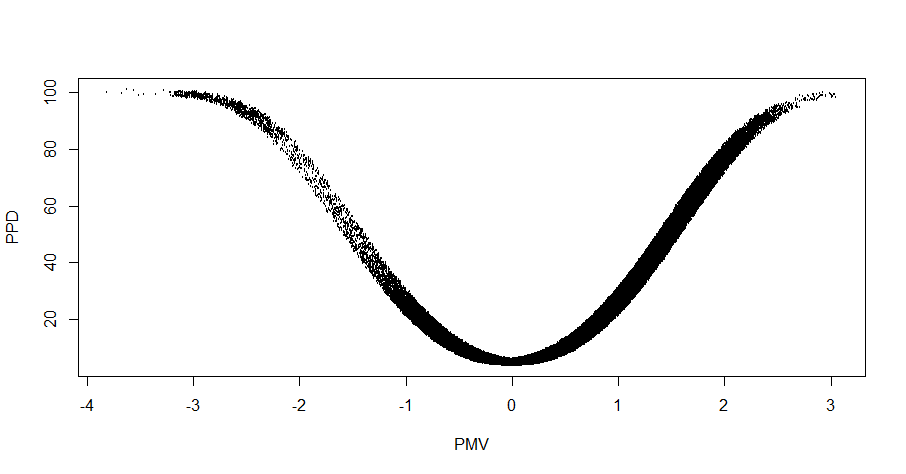
\includegraphics[scale=0.52]{Images/GainsMetPMVPPD/PMVvsPPD}
\caption{Relation entre les indices PMV et PPD}
\label{fig:PMVvsPPD}
\end{figure}

La connaissance de la sensation thermique des occupants n'est pas une information directement nécessaire pour l'outil de simulation thermique. Néanmoins cette information est, au même titre que la connaissance des activités, nécessaire à la modélisation des activités adaptatives, tel que la gestion du chauffage.

\section{Gestion des ouvrants}

\subsection{État de l'art}

Le contrôle de l'ouverture et fermeture des fenêtres est un paramètre fondamental du confort adaptatif et de la consommation énergétique des bâtiments. Une prise en compte affinée de cette gestion est alors nécessaire à un exercice de prédiction. Pour cela, nous avons pu recenser dans la littérature un nombre de propositions de modèles très élevé, que nous présentons dans ce présent chapitre. Le Tableau \ref{tab:WinPres} synthétise le contexte de la campagne de mesure, le type de modèle ainsi que les atouts et faiblesses du modèle proposé. Pour sa part, le Tableau \ref{tab:WinInOut} met en avant les variables d'entrée et de sortie des différents modèles. Nous proposons également une présentation succincte du fonctionnement des modèles dans les paragraphes ci-dessous.

Bien que la corrélation entre les actions sur les fenêtres et les températures internes et externes ait été établie depuis les premières fenêtres, le premier modèle mathématique de prédiction a été proposé en 1984 par Warren et Parkins \cite{Warren-84}. Dans ce modèle la proportion de fenêtres ouvertes dépend de la météo (2 niveaux: ensoleillé ou nuageux), de la taille des ouvrants (2 niveaux: grands ou petit) et de la température extérieure (régression linéaire). Warren et Pakins assurent que les actions sur les petites fenêtres sont motivées par la qualité de l'air et que les actions sur les baies sont davantage liées au confort thermique.

Fritsch et al. \cite{Fritsch-90} proposent un modèle pour prédire l'angle d'ouverture des fenêtres en hiver. Lors des heures de travail un processus de Markov définit les probabilités de transition (chaque 30 minutes) entre 6 angles d'ouvertures possibles sur 4 plages de température.

Nicol \cite{Nicol-01} est le premier à corréler la température extérieure avec la proportion de fenêtres ouvertes par une régression logistique. Il réalise ce travail sur des bureaux localisés en Europe, en Angleterre et au Pakistan. Il note que les pakistanais ont tendance à moins ouvrir les fenêtres que les 2 autres groupes, qu'il explique par un contexte différent (bureaux climatisés, air sec, contrôle sur les fenêtre limité, ...).

Yun et Steemers  \cite{Yun-08} proposent un modèle qui considère la présence (arrivées et départs) des occupants pour estimer la probabilité d'action sur les ouvrants. L'ensemble des modèles revus utilise la température extérieure comme variable explicative principale, plutôt que la température extérieure, car c'est une variable dépendante du site uniquement et pas du bâtiment modélisé. Une autre difficulté à l'utilisation de la température interne est sa relative invariance en période de chauffe, ce qui mène à une corrélation non significative avec la position des fenêtres en hiver. Néanmoins, Yun et Steemers se sont restreint à la période estivale et suggèrent clairement que l'action sur les fenêtres est principalement expliquée par la température interne. De plus, il est observé dans cette étude que pour des raisons de sécurité l'ensemble des fenêtres étaient fermées la nuit, exceptées celles qui avaient été conçues de sorte à ce que la ventilation naturelle soit exploitée.

Rijal et al. \cite{Rijal-08} proposent un modèle plus raffiné qui considère la température opérative et externe. Ils utilisent une régression logistique multiple pour définir la probabilité d'ouverture d'une fenêtre. Une bande morte de $\pm 2K$ pour la température intérieure et de $\pm 5K$ pour la température extérieure est définit pour différentier les probabilités d'ouverture de celles de fermetures et donc éviter une répétition d'actions. En ayant pré-calculé les températures externes, opérative et de confort, la probabilité d'action est calculée par $logit(p)=0.171\theta_{op}+0.166\theta_{out}-6.4$, si $|\theta_{op}-\theta_{confort}|>2K$. L'ensemble de ce modèle est plus connu sous le nom d'algorithme d'Humphreys et est disponible dans la version standard du logiciel ESP-r. 

Comme Yun et Steemers \cite{Yun-08}, Herkel et al. \cite{Herkel-08} considèrent les déplacements des occupants entre zones comme une variable explicative de la gestion des ouvrants. En revanche, ce modèle utilise des chaines de Markov pour définir les déplacements, puis des probabilités de transitions déterminées par régressions logistiques fonction de la température extérieure pour déterminer l'action sur la fenêtre.

Les probabilités d'actions dans le "meilleur" modèle d'Haldi et Robinson \cite{Haldi-09} dépendent des mouvements des occupants entre zones, mais également de variables environnementales et contextuelles. Ces dernières sont composées de 2 booléens indiquant s'il pleut et si la zone se trouve au rez-de-chaussé. Les auteurs de ce modèle sont à notre connaissance les premiers à avoir proposé en addition des probabilités de transition d'état, des durées d'ouvertures dépendantes uniquement de la température extérieure.

Schweiker et al. \cite{Schweiker-12} sont à notre connaissance les premiers à avoir proposé un modèle robuste de gestion des ouvrants dans le secteur résidentiel pour les chambres et pièces à vivre. Ils ont testé la performance du modèle d'Haldi et Robinson \cite{Haldi-09} sur des appartements en Suisse et une résidence étudiante au Japon et ont conclu que les prédictions pour les logements Suisse étaient acceptables contrairement aux mesures sur la résidence asiatique. Les raisons avancées au non-fonctionnement sont le climat chaud et humide, l'utilisation d'air conditionné et la forte absence des étudiants en journée. Il est à noter que les mouvements entre zones ne sont pas considérés, à cause de l'impossibilité de définir des transitions d'occupation précises.

Zhang et Barret \cite{Zhang-12} ont testé la sensibilité des facteurs d'influences sur la gestion des ouvrants par les occupants. Bien que les résultats de recherche listent les facteurs d'influences, les auteurs ne présentent pas de modèle pouvant être intégré à un outil de simulation thermique.

Andersen et al. \cite{Andersen-13} ont proposé un modèle de gestion des ouvertures dans les chambres et pièce à vivre de logements. Les auteurs ont différentié les logements habités par des propriétaires et des locataires ainsi que les logements ventilés mécaniquement et naturellement, formant 4 groupes. Pour chacun de ces groupes la période de la journée, la saison et d'autres facteurs environnemental sont intégrés à des modèles logistiques selon leurs influences. 

Fabi et al. \cite{Fabi-14} ont étudié les facteurs d'influence des actions sur les ouvrants de différents bureaux et indiquent qu'il est difficile de trouver un consensus sur les paramètres les plus influents. Même la température extérieure n'apparait pas influente sur l'ensemble des bureaux avec seulement 1 bureau sur 7 pour les ouvertures et 5 sur 7 pour les fermetures. Le paramétrage pour une intégration dans un outil de simulation n'est pas fournit.

D'Oca et al. \cite{d'Oca-14} reprennent la suite des travaux d'Andersen et al. \cite{Andersen-13} sur de la modélisation en résidentiel et proposent un modèle d'ajustement de température de consigne en plus de la gestion des ouvrants. Les auteurs suggèrent d'intégrer de la diversité entre les occupants modélisés, sans pour autant donner plus de détails.

\begin{landscape}
\begin{table} [H]
\begin{tabular}{|p{2.5cm}|p{2cm}|p{2cm}|p{2cm}|p{2cm}|p{2cm}|p{4cm}|p{4cm}|}
\hline 
Auteurs & Location & Bâtiment & Durée campagne & Intervalle de mesure & Modèle & Points forts & Points faibles \\ 
\hline 
\hline
Warren et Parkins \cite{Warren-84}, 1984 & Royaume-Uni & 5 bureaux & 3 mois & 2 fois/jour & Régression linéaires & Distinction des ouvrants par leurs tailles & Modèle statique \\ 
\hline 
Fritsch et al. \cite{Fritsch-90}, 1990 & Suisse & 4 bureaux & 8 mois & 30 min & Processus de Markov & 6 angles d'ouverture estimés & Restriction à la saison de chauffe; Pas de temps élevé \\ 
\hline 
Nicol \cite{Nicol-01}, 2001 & Pays européen et Pakistan & 25 bureaux & ? & ? & Régression logistique & Nature internationale des données & Modèle statique; Variable explicative unique \\ 
\hline 
Yun et Steemers  \cite{Yun-08}, 2008 & Royaume-Uni & 6 bureaux & 3 mois & 30 min & Régression logistique & Considération des mouvements des occupants & Restriction à la période estivale \\ 
\hline 
Rijal et al. \cite{Rijal-08}, 2008 & Royaume-Uni & 15 bureaux & 18 mois & 15 min & Régression logistique & Température opérative considérée & Base de données ancienne; Calibration bande morte \\ 
\hline 
Herkel et al. \cite{Herkel-08}, 2008 & Allemagne & 21 bureaux & 13 mois & 1 min & Régression logistique & Saisonnalité considérée & Fréquence de transition sur-évaluée; Paramétrage non-fournit \\ 
\hline 
Haldi et Robinson \cite{Haldi-09}, 2009 & Suisse & 14 bureaux & 7 ans & 5 min & Régression logistique + Weibull & Comparaison de 8 modèles; Validation interne & Angle d'ouverture non considéré \\ 
\hline 
Schweiker et al. \cite{Schweiker-12}, 2012 & 1)Suisse; \newline 2)Japon & 1)3 appart.; \newline 2)39 dortoirs & 1)16 mois;\newline 2)1 mois & 1 min & Bernoulli; Markov; Humphreys & Validation externe de \cite{Haldi-09} et \cite{Rijal-08}; Extrapolation sur le résidentiel & L'influence de l'occupation n'est pas utilisée \\ 
\hline 
Zhang et Barret \cite{Zhang-12}, 2012 & Royaume-Uni & bureaux & 16 mois & 60 min & Modèle logistique & Étude de l'orientation; Considération des espaces communs & Variable explicative unique alors que davantage sont significatifs \\ 
\hline 
Andersen et al. \cite{Andersen-13}, 2013 & Danemark & 15 logements & 8 mois & 10 min & Régression logistique & Statut d'occupation (propriétaire/locataire) étudié & Moins d'une année de mesure; peu parcimonieux (4 sous-modèles) \\ 
\hline 
Fabi et al. \cite{Fabi-14}, 2014 & République Tchèque & 8 bureaux & 11 mois & 5 min & Régression logistique & Diversité entre occupants & Pas de validation \\ 
\hline 
D'Oca et al. \cite{d'Oca-14}, 2014 & Danemark & 15 logements & 8 mois & 10 min & Régression logistique & Diversité entre occupants & L'occupation n'est pas utilisée \\ 
\hline 
\end{tabular}
\caption{Synthèse des modèles les plus pertinents de gestion des ouvrants}
\label{tab:WinPres}
\end{table}
\end{landscape}

\begin{table} [H]
\centering
\begin{tabular}{|l||c|c|c|c|c|c|c|c|c|c|c|c|}
\hline
\textbf{Variables\textbackslash Auteurs} & \cite{Warren-84} & \cite{Fritsch-90} & \cite{Nicol-01} & \cite{Yun-08} & \cite{Rijal-08} & \cite{Herkel-08} & \cite{Haldi-09} & \cite{Schweiker-12} & \cite{Zhang-12} & \cite{Andersen-13} & \cite{Fabi-14} & \cite{d'Oca-14}\\
\hline
\hline \rowcolor{gray}\textbf{Environnementales} & \multicolumn{12}{c}{} \\
\hline Température intérieure / opérative &  & / &  & X & X & / & X & X & / & / & X & X \\
\hline Température extérieure & X & X & X & / & X & X & X & X & X & X & X & X \\
\hline Rayonnement solaire & X & / &  &  &  & / &  &  & / & / &  & X \\
\hline Vitesse du vent & / & / &  &  &  & / &  & / & / &  &  & / \\
\hline Précipitation & / & / &  &  &  &  & X &  & / &  &  &  \\
\hline Bruit &  & / &  &  &  &  &  &  &  &  &  &  \\
\hline Odeur et polluants &  & / &  &  &  &  &  &  &  & X &  & / \\
\hline Humidité &  & / & / &  & / &  &  & / & / & / & X & / \\
\hline Saisonnalité &  &  &  &  &  &  &  &  & X & / & / &  \\
\hline Heure de la journée &  &  &  & / &  &  &  &  & X & / & / & X \\
\hline \rowcolor{gray}\textbf{Socio-psycho-physiologiques} & \multicolumn{12}{c}{} \\
\hline Mouvements occupants et activité &  & / &  & X &  & X & X &  & / &  & X &  \\
\hline Propriétaire/Locataire &  &  &  &  &  &  &  &  &  & / &  &  \\
\hline Espace partagé &  &  &  &  &  &  & / & / &  &  & / &  \\
\hline Sécurité (Étage) &  &  &  & / &  &  & X &  &  &  &  &  \\
\hline Différences culturelles &  &  & / &  &  &  &  & / &  &  &  & / \\
\hline \rowcolor{gray}\textbf{Bâti et système} & \multicolumn{12}{c}{} \\
\hline Type / Taille d'ouvrant & X &  & / &  &  &  &  &  &  &  &  &  \\
\hline Type / Taille de la pièce &  &  &  &  &  &  &  &  &  & / &  & X \\
\hline Orientation &  &  &  &  &  &  &  &  & / &  &  &  \\
\hline Air conditionné &  &  & / &  &  &  &  & X &  &  &  &  \\
\hline Ventilation mécanique &  &  &  &  &  &  &  &  &  & / &  &  \\
\hline \rowcolor{gray}\textbf{A expliquer} & \multicolumn{12}{c}{} \\
\hline Etat ouvert/fermé & X & & X & & & & & & & & &  \\
\hline Probabilité d'action &  & X & & X & X & X & X & X & X & X & X & X \\
\hline Angle d'ouverture &  & X &  &  &  &  &  & X &  &  &  &  \\
\hline
\end{tabular}
\caption{Synthèse des données d'entrée et de sortie des modèles de gestion des ouvrants étudiés}
\label{tab:WinInOut} 
\end{table}

A partir de cette revue de modèles de gestion des ouvrants, nous pouvons tirer plusieurs conclusions:
\begin{itemize}
\item peu d'études ont été réalisées dans les logements,
\item les régressions logistiques et les processus de Markov à temps discret sont les modèles les plus fréquemment utilisés,
\item les stimulus thermiques sont la cause prédominante des actions sur les ouvrants,
\item les arrivés et départs entre pièces favorisent les actions,
\item la saisonnalité a un impact significatif sur la gestions des ouvrants, mais semble étroitement corrélée à la température extérieure,
\item la taille des fenêtres et l'angle d'ouverture sont rarement considérés,
\item les relations sociales sur le choix de l'état de la fenêtre sont peu documentées,
\item les études sont indépendantes et peu de procédures de validations externes existent, 
\item le climat, le type d'utilisation et la présence d'air-conditionné ont une influence déterminante sur l'action des ouvrants,
\end{itemize}

\subsection{Modèle d'Haldi et Robinson}
\label{Modèle d'Haldi et Robinson}

 Le modèle de base utilisé dans la plateforme pour prédire les interactions avec les fenêtres est celui d'Haldi et Robinson \cite{Haldi-09}. Ce modèle hybride prédit dans un premier temps les probabilités de transition du modèle de Markov issues de régression logistiques, puis en cas d ouverture prédit la durée d'ouverture de la fenêtre issue d'une distribution de Weibull.

La probabilité de transition est composée de modèles non imbriqués, ou \textit{non-nested} en anglais, de la forme:

\begin{equation}
P_{ij}(x_{1},...,x_{n})=\frac{exp(\alpha + \Sigma^{n}_{k=1}\beta_{k}x_{k})}{1+exp(\alpha + \Sigma^{n}_{k=1}\beta_{k}x_{k})}
\label{Pij}
\end{equation}

Le modèle de gestion des ouvrants est en réalité composé de sous-modèles qui dépendent de la présence des occupants. Le modèle diffère alors selon que l'occupant arrive dans une zone, qu'il y soit de façon intermédiaire ou qu'il en parte. Nous pouvons noter que la connaissance de $P_{10,int}$ et de $P_{10,arr}$ n'est pas nécessaire puisque dans ces cas la durée d'ouverture a déjà été attribué et la fenêtre se fermera une fois le décompte achevé. Le Tableau \ref{coefWindows} synthétise les coefficients associés aux autres probabilités.

\begin{table} [H]
\begin{tabular}{|c||c|c|c|c|c|c|c|c|c|}
\hline 
 & $\alpha$ & $\beta_{\theta_{in}}$ & $\beta_{\theta_{out}}$ & $\beta_{\theta_{out,dm}}$ & $\beta_{f_{abs,prev}}$ & $\beta_{f_{abs,next}}$ &  $\beta_{t_{pres}}$ & $\beta_{R}$ & $\beta_{GF}$  \\ 
\hline 
\hline
$P_{01,arr}$ & -13.88 & 0.312 & 0.0433 & 0 & 1.862 & 0 & 0 & -0.45 & 0 \\ 
\hline 
$P_{01,int}$ & -12.23 & 0.281 & 0.0271 & 0 & 0 & 0 & -8.78.10$^{-4}$ & -0.336 & 0 \\ 
\hline 
$P_{01,dep}$ & -8.75 & 0 & 0 & 0.1371 & 0 & 0.83 & 0 & 0 & 0 \\ 
\hline 
$P_{10,dep}$ & -8.54 & 0.21 & 0 & -0.09 & 0 & 1.61 & 0 & 0 & -0.92 \\ 
\hline 
\end{tabular} 
\label{coefWindows}
\caption{Coefficients des variables explicatives des probabilités de transition des ouvertures de fenêtres}
\end{table}

Lorsque le modèle prédit une ouverture, une distribution de la durée d'ouverture est estimée par la distribution de Weibull. L'équation permettant de déterminer la durée d'ouverture est:

\begin{equation}
t_{open}=-\lambda.log(random)^{\frac{1}{k}}
\label{distWeibull}
\end{equation}

avec les paramètres de forme $k=0.418$ et d'échelle $\lambda=\frac{1}{e^{(2.213+0.173\theta_{out}})}$, $random$ un nombre aléatoire entre 0 et 1 et $\theta_{out}$ la température extérieure, et seule variable explicative de loi de Weibull. La Figure \ref{fig:WeibullTest} permet de visualiser son impacte sur la durée d'ouverture des fenêtres. Ainsi, on peut lire que pour un même nombre aléatoire généré la durée d'ouverture sera d'autant plus longue que le température extérieure sera élevée.

\begin{figure}[H]
\centering
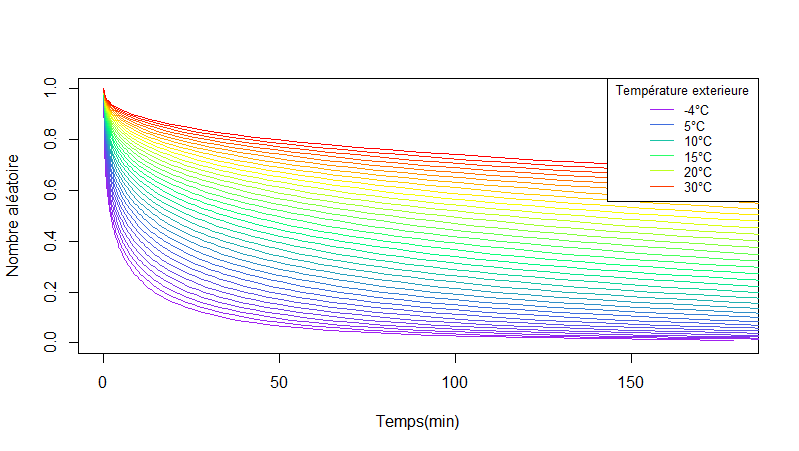
\includegraphics[scale=0.6]{Images/Fenetre/WeibullTest}
\caption{Fonction de survie de la durée d'ouverture suivant la fonction de Weibull pour des températures extérieures comprises entre -4 et 32 $^{\circ}$ C}
\label{fig:WeibullTest}
\end{figure}

\subsection{Ajustement du modèle}

 Fabi et al. \cite{Fabi-12}
Incorporation de phénomènes sociologiques qualitatifs au modèle:
By default the regression coecient k parameters used with the
predictors in equation 4.1.5 are estimated from data relating to an aggregate population (ie.
using all empirical data for all members of the population surveyed), so that each agent will
uses the same values to predict the probability of a transition
    - Lorsque l'activité cuisine a lieu on ouvre la fenêtre
    - Lorsque l'occupant se réveille alors il ouvre la fenêtre
    - Intégration des PMV ou PPD
    - Dans le modèle de base, lorsque l'occupant entre dans la pièce et que la fenêtre est ouverte alors la durée d'ouverture est calculée. Une idée consiste alors de considérer le confort thermal.
Andersen et al. \cite{Andersen-13} on avancé l'hypothèse que les fumeurs ouvrent plus la fenetre.
    
\section{Gestion des stores}

1- Etat de l'art sur les drivers de la gestion des stores
La these d'Haldi peut être reprise pour cette partie
L'éblouissement est un driver important pour la gestion des stores. Néanmoins, l'éblouissement est difficilement exprimable numériquement il est donc peu évident de l'intégrer dans les outils de simulation.

2- Présentation du modèle courant

3- Incorporation de facteur contextuels qualitatifs au modèle:
	- Lorsque l'activité audio-visuelle a lieu on ferme les stores
	- Lorsque l'activité dormir a lieu on ferme les stores
	- Intégration des PMV ou PPD
	- Store intérieur, rideaux ou extérieur?
	
\section{Gestion de l'éclairage}
\label{Gestion de l'éclairage}

1- Présentation du modèle courant

2- Incorporation de phénomènes sociologiques qualitatifs au modèle:
	- Lorsque l'activité audio-visuelle a lieu on ferme la lumière
	- Lorsque l'activité dormir a lieu on éteins forcément la lumière

\section{Utilisation des appareils électriques}

\subsection{Types d'appareils électriques}

Widén (2009) a catégorisé les appareils électriques en fonction de l'utilisation de la puissance:
\begin{table} [H]
\centering
\begin{tabular}{|l||l|}
\hline Type de puissance & Exemple \\
\hline
\hline Puissance non définie par l'activité & Appareils de froid, radio réveil \\
\hline Puissance constante pendant l'activité & Télévision, Appareils de cuisson \\
\hline Puissance constante après l'activité & Machine à laver, lave vaisselle \\
\hline Puissance constante après avec contrainte de temps & Bains, douches \\
\hline Activité avec puissance dépendante du temps & Éclairage (variations journalières et de saison) \\
\hline 
\end{tabular}
\end{table}
Une catégorisation de la sorte permet une étude temporelle de la variation d'énergie.

\subsection{Modélisation de la possession et de l'utilisation des appareils électriques}

Jaboob (2015) propose une modélisation du taux de pénétration \footnote{Le taux de pénétration aussi appelé taux d'équipement est le pourcentage de la population équipée d'un appareil électrique}de la possession, de l'utilisation et de la fraction de puissance des appareils électriques. Cette modélisation est de type bottom-up pour chaque famille d'appareil, cela permet de considérer la diversité des ménages, des comportements individuels des occupants et bien sûr les caractéristiques intrinsèques des appareils. La modélisation de la possession des appareils est réalisée par régression logistique. La modélisation de l'utilisation des appareils considère d'une part l'allumage et d'autre part sa durée d'utilisation. L'allumage est modélisé par Bernoulli et la durée par un processus aléatoire à temps continu. La modélisation de la fraction de la puissance est réalisée par processus de Bernoulli ou de Markov.

\section{Gestion des consignes de température}

Intégrer quelque part \cite{d'Oca-14} - Voir le réutiliser.

1- Que cherche t-on? Prédire la température de consigne pour l'envoyer au cœur de calcul.

2- Introduction sur le choix de la température de chauffage (Brisepierre, p273 - sociologie de l'energie]

3- Comment la température de consigne est utilisée par EnergyPlus? En étudiant la température intérieure on s'aperçoit qu'elle est strictement égale à la température de consigne. Hypothèse également faite par le CEREMA dans ces travaux sur le suivi de bâtiments démonstrateurs à basse consommation. (p127  Bat démonstrateurs à basse consommation d'énergie - Enseignements opérationnels tirés de 60 constructions et rénovations du programme PREBAT 2012-2015). "L'analyse statistique des températures en période de chauffe permet d'estimer la température en hiver en se basant sur la mesure de la température intérieur pendant les heures de fonctionnement du chauffage et pendant les heures d'occupation identifiées par enquête."

4- Quels sont les facteurs influençant l'utilisation des systèmes de chauffage.

Plusieurs études ont recensé les facteurs influençant l'utilisation des systèmes de chauffage. L'Annex53 \cite{Annex-53-1} a synthétisé l'ensemble de ces facteurs d'un point de vu qualitatif. Maresca et al. \cite{Maresca-09} ont pour leur part réalisé une étude pour le compte du CREDOC sur la maîtrise des consommations d'énergie des ménages. L'approche sociologique par plan d'expérience est pleine d'enseignements, cette approche permet notamment de déterminer avec un minimum d'essai l'influence individuel des différents paramètres. Dealière et al \cite{Devaliere-11} dans l'article de l'INSEE - La précarité énergétique: avoir froid ou dépenser trop pour se chauffer - justifient les différences de satisfaction thermique selon des variables propres au ménage, comme le revenu et sa structure, mais également par la vétusté du logement et le système de chauffage. Cavailhes et al.\cite{Cavailhes-11} de l'INRA  ont utilisé des méthodes d'économétrie de données de panel issues des enquêtes logement de l'INSEE. Cette étude considère l'ensemble des variables explicatives généralement avancé mais présente ses résultats sous forme d'évolution entre les années de référence de l'étude, 1984 et 1988, ce qui les rend difficilement exploitable dans notre contexte. Penot-Antoniou et al. \cite{Penot-Antoniou-13} dans le rapport sur les déterminants de la température de chauffage, analysent la variance entre la température adoptée par les ménages et les variables explicatives qualitatives. L'approche est celle qui correspond au besoin, car elle laisse la possibilité d'être codé et intégré à notre plateforme comportementale, en revanche un certain nombre de paramètres issus de l'étude économétrique ont des coefficients difficilement explicables. Par exemple un ménage ayant des ressources comprises entre 535 et 1100 \euro se chauffe de 2.5 \degre C de plus que la moyenne alors qu'un ménage gagnant de 1100 à 1500 \euro se chauffe moins de 1.7 \degre C en moyenne. Ce résultat non linaire n'est pas une exception et soulève un doute sur la fiabilité de l'étude, qui se repose pourtant sur un échantillon de 373 ménages.

\cite{Kelly-13} : Complexe mais parcimonisation envisageable

\cite{Andersen-09} : Petite étude sur 13 logements

\cite{Fabi-13}: Même données qu'Andersen mais développement d'un modèle logistique plutôt que linéaire.


\begin{table} [H]
\centering
\begin{tabular}{|l||c|c|c|c|c|c|c|}
\hline
\textbf{Variables \textbackslash Auteurs} & \cite{Annex-53-1} & \cite{Maresca-09} & \cite{Devaliere-11} & \cite{Cavailhes-11} & \cite{Penot-Antoniou-13} & \cite{Kelly-13} & \cite{Andersen-09} \\
\hline
\hline \rowcolor{gray}\textbf{Environnementales} & \multicolumn{7}{c}{} \\
\hline Zone climatique & & & & X & X & & \\
\hline Température extérieure & X & & & & & X & X \\
\hline Humidité relative / Pluie & X & & & X & & & X \\
\hline Altitude & & & & X & & & \\
\hline Vitesse du vent & X & & & & & & X \\
\hline Radiation solaire & & & & & & & X \\
\hline Localisation / Type de commune & & X & & X & & X & \\
\hline Heure de la journée & X & & & & & & X \\
\hline \rowcolor{gray} \textbf{Socio-psychologique} & \multicolumn{7}{c}{} \\
\hline Statut d'occupation & X & & X & X & X & X &  \\
\hline Revenu & & X & X & & X & X & \\
\hline Age & & X & & X & X & X & \\
\hline Nationalité & & & & X & & & \\
\hline Diplôme & & & & X & & & \\
\hline Genre & X & & & X & & & \\
\hline Coût du chauffage & & & X & X & & & \\
\hline Structure du ménage / CO2 & & & X & & X & X & X \\
\hline Vêture & X & & & & & & \\
\hline Stratégie de régulation & X & & & & & X & \\
\hline \rowcolor{gray}\textbf{Bâti et systèmes} & \multicolumn{7}{c}{} \\
\hline Année de construction & & X & X & X & X & X & \\
\hline Travaux de réhabilitation & & & & & X & & \\
\hline Type de chauffage & & & X & X & X & X & \\
\hline Type de combustible & & & & & X & X & \\
\hline Qualité enveloppe & X & & X & X & X & X & \\
\hline Structure du bâti (individuel/collectif) & & X & X & & & X & \\
\hline Exposition principale & & & & X & & & \\
\hline Superficie & & X & & X & & & \\
\hline Étage & & & & X & & & \\
\hline Pièces du logement & & X & & & & & \\
\hline Type de ventilation & X & & & & & & \\
\hline 
\end{tabular}
\end{table}

D'autres modèles ont été développé comme l'analyse statistique de Karjalainen -----CITE----- sur l'utilisation des thermostats en Finlande ou la régression linéaire multivariée de Schweiker et al. sur la modélisation de l'air conditionné au Japon... <- T. Hong, An Ontology to represent energy ....

Notre choix se porte sur le modèle de Kelly et al. car il est basé sur une étude significative, car ...

5- Choix pour le modèle de Kelly. Avec adaptation pour un modèle plus parcimonieux.

Pour développer un modèle, de type régression linéaire multiple, un logiciel de programmation statistique - comme R - a été utilisé. Ce type de logiciel permet de déterminer les coefficients Alpha et $a_{i}$ de l'équation de régression:

\begin{equation}
T_{int} = Alpha + \sum\limits_{i=1}^n a_{i} * V_{i} 
\end{equation}

Avec $T_{int}$ la température intérieure journalière, $Alpha$ et $a_{i}$ les coefficients à déterminer pour la régression et $V_{i}$ les valeurs des variables explicatives.

Pour obtenir les différents coefficients sous R il suffit de rentrer la fonction lm() en y spécifiant la variable à expliquer, les variables explicatives et la localisation du fichier:
\begin{verbatim}
   lm(Tint ~ Text + Text2 + Localisation + ... + Dbl_Glz + Wall_U, data = mydata)
\end{verbatim}

Le logiciel R génère alors les coefficients de la régression et 

Au risque de 1\%, il n'existe pas d'association statistiquement significative entre la température intérieure et les variables explicatives: déclaration de température de consigne, présence d'un programmateur automatique, tranche d'age de 60-64 ans, présence d'un système de chauffage central et d'un système de chauffage au gaz d'appoint. Ces variables explicatives sont donc supprimées du modèle développé.

Nous proposons aussi dans le fichier de configuration de laisser la possibilité aux utilisateurs de ne pas définir certains paramètres lorsqu'ils ne sont pas connus!

6- Changement de la température intérieure

\cite{Fabi-13}
Le modèle résulte en de petits ajustements de la température de consigne. Cela est en adéquation avec les résultats de l'étude d'Andersen \cite{Andersen-09} qui indique que les actions adaptatives des habitants lorsqu'ils ont froid sont de 66 à 78 \% du temps de petits ajustement contre moins de 5\% du temps des grosses augmentations sur le thermostat.

7- Interactions sociales ...

Le modèle de base de Kelly peut être complété par l'incorporation d'informations qualitatives supplémentaires

La température de consigne fixée à 19 \degre C depuis le choc pétrolier de 1974 fait figure de norme mais ne reflète pas les faits réels. Son influence sur les consommations énergétiques y est très fortement corrélé et un ajustement plus fidèle à la réalité est nécessaire.
Pour cela le modèle proposé consiste à tirer sur une loi normale la température de base issue du bureau d'études d'Enertech. Puis, en fonction des paramètres d'influences V (age, genre, charge financière, zone, longue absence...) la base est modifiée:

\[T_{consprinc}=T_{base}+\sum_{V}X_{V}\]

Cette approche proposée par Vorger \cite{Vorger-14} est très souple et permet notamment de gérer les réduits. Son calibrage est néanmoins discutable car basé sur le bon sens. En ce basant sur le \textit{British Home Heating Study} qui a réalisé une enquête sur les systèmes de chauffage et de contrôle, un modèle sur le choix de la température de consigne, notamment en fonction du systèmes, peut être créé plus finement. Cette enquête est composée d'un questionnaire et de mesures dynamiques (températures, humidité relative, ...) sur un échantillon de 32 familles anglaises.

Manque de données nous oblige à adopter une approche empirique, plutôt que de ré-exploiter des modèles qui ne nous semble pas robustes. Le modèle proposé a donc vocation à être amélioré, lorsque des données sur la fréquence des interactions des occupants avec le système de chauffage seront disponibles.

Mise en contexte:
- Intégration des PMV ou PPD

\section{Consommations d'eau chaude sanitaire}

\subsection{Systèmes}

Le modèle d'ETI ainsi que des données nationales (A trouver INSEE) peut permettre de modéliser les systèmes de chauffage de l'eau et le taux de pénétration des systèmes. Cette modélisation préalable est souvent omise dans les modèles de puisages d'ECS alors que son impacte sur les consommations finales en dépend relativement significativement.

On recense trois principales énergies pour la production d'eau chaude sanitaire: le gaz, l'électricité et les énergies renouvelables. Les chauffes-eau au gaz et électriques sont soit instantanés soit à accumulation. Concernant les énergies renouvelables, on retrouve de manière croissante le ballon thermodynamique ou pompe à chaleur et le chauffe eau solaire d'appoint.

\subsection{Volumes de consommation}

Selon Evarts et Swan \cite{Evarts-13} les puisages d'ECS sont très diverses selon les ménages et donc dépendent de leurs caractéristiques socio-démographiques. La fréquence et l'intensité des puisages sont encore plus fortement corrélés aux activités des occupants.

Selon les activités en cours, des puisages d'ECS y sont associés. A titre d'exemple, l'activité nettoyage corporelle implique un puisage en lien avec celui de la douche ou du bain.

L'ADEME a lancé un programme de recherche, baptisé PACTE, pour améliorer l'efficacité énergétique de l'ECS dans l'habitat. Ces travaux visent à améliorer la prise en compte de la dimension socio-comportementale de l'usage de l'ECS et à modéliser, simuler et évaluer le fonctionnement des équipements. La figure \ref{fig:PACTEECS} présente les partenaires du PACTE ECS, dont l'investissement est de plus 8 millions d'euros sur 5 ans.

\begin{figure}[H]
\centering

\includegraphics[scale=0.8]{Images/PACTEECS}
\caption{Les différents partenaires du PACTE ECS}
\label{fig:PACTEECS}
\end{figure}

La figure \ref{fig:Foisonnement_ECS} révèle la diversité de consommation à l'échelle du logement plutôt qu'à celle d'un immeuble.

\begin{figure}[H]
\centering
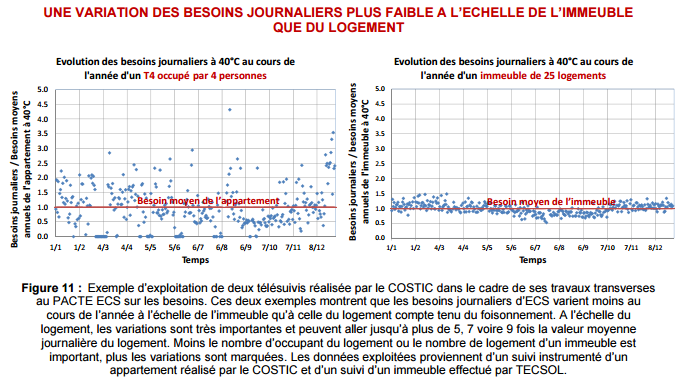
\includegraphics[scale=0.9]{Images/Foisonnement_ECS}
\caption{Importance de l'information à l'échelle du logement pour prendre en compte la diversité des consommations}
\label{fig:Foisonnement_ECS}
\end{figure}

La publication ADEME-COSTIC des résultats valorisés est prévue courant 2016 alors que l'étude se tient depuis 2011.

Contacter le directeur technique de COSTIC: Cedric Beaumont (prestations@costic.com) pour récupérer les résultats non agrégés 




%%%%%%%%%%% A intégrer quelque part!
% Plessis et al. \cite{Plessis-14} introduisent la notion de confort du groupe qui est utilisée pour déterminer quel action le groupe choisi (ex: augmenter la température, ouvrir la fenêtre). En opposition aux actions individuels (adaptation de l'habillement, changement d'activité).

%Schweiker \cite{Schweiker-16} a étudié les interactions entre les occupants et le bâtiments. Il a constaté que les occupants de bureaux partagés ont tendance à moins modifier leur environnement que les occupants de bureaux individuels. 